\section{Background}
John Maynard Keynes work revolutionized economic thought; however, he never formalized any of his theories into a mathematical theory. This was performed in a process known as the neoclassical synthesis which was so called for its attempt to bridge classical models with these Keynesian principles. Paul Samuelson and Sir John Hicks were deeply influential in summarizing Keynesian macroeconomics into mathematically tractable models and their work was incorporated into a discrete-time business cycle model by T\"{o}nuu Puu\autocite{Puu2003}. Key to the theory of the model are the concept of a multiplier and accelerator.

Keynes espoused the idea that increasing spending in the economy by some amount $x$ actually increased the national output by an amount $>x$. In essence, the effect of increased spending was actually multiplied by a positive amount. Although this was originally studied in order to determine the effects of changes in government spending in order to inform fiscal policy\autocite{Samuelson1939}, the principle of the mechanism impacts all forms of expenditure in the economy. 

Integral to the rise of cyclic dynamics in the model is the presence of the Keynesian accelerator which actually makes use of the multiplier effect. The effect can be best explained via example: suppose there is a general increase in national output level. This increases business profits and expectations, thus inducing them to increase investments. This further increases output via the multiplier effect, causing an accelerating level of growth. The same occurs if the economy depresses as businesses will decrease investment due to falling prospects\autocite{Jorgenson1963}

The combination of these two mechanisms, typically referred to as the multiplier-accelerator effect, are sufficient in creating a stable cyclic or even chaotic economy as opposed to a static steady-state model. This type of model allows for cyclic behavior to occur endogenously, that is to say the model allows for persistent behavior outside of the steady state. This idea runs contrary to the idea that economic booms and recessions are reactions to exogenous shocks which is common in the new classical models. Also known as freshwater economics, these models assume that agents are perfectly rational and are capable of learning from past experiences. This viewpoint came into prominence in the late 1970s with a model by Lucas and Sargent\autocite{Lucas1979} which sought to move past these seemingly outdated Keynesian principles. In the modern day however, Keynesianism has regained popularity with a new neoclassical synthesis that resulted in a new school of thought, New Keynesianism, that seeks to provide stronger micro-foundations to macroeconomic models than was previously encountered in neo-Keynesianism. 
\section{Model Set-up}
The model presented here is identical to that presented by T\"onu Puu\autocite{Puu2003}. The first factor of the economy to consider is that of investment, $I$. In order for investment to operate under Keynes' accelerator principle, capital stock must be in a proportion to the change in income, thus the investment level would be a function of the rate of change in income. 

A linear function for investment captures this premise; however, this leads to unrealistic behavior for higher magnitudes of income change. Suppose income dramatically increased; a linear function implies that a proportionally high level of investment can sustain this higher level of production when in reality other factors of production such as the land, labor, or technology available are the primary limiting factors. Of larger concern with a linear model though is if the economy encounters a sharp decrease in income. This induces a large, negative value for investment which implies that firms would actively destroy their machinery and other forms of capital stock in the event of an economic recession. This is obviously unrealistic and so John Hicks introduced a piecewise linear investment function such that at extreme levels of income change, investment will reach a predetermined maximal or minimal value. This piecewise function was then adapted to be differentiable over all points by Richard Goodwin by approximating the curve with a hyperbolic-tangent function\autocite{Puu2003}.

Puu approximates the hyperbolic-tangent function with its linear-cubic Taylor series expansion as this introduces a back-bending behavior into the curve. This allows the investment curve to capture not only firm behavior in the private sector but also implicitly include government spending and taxation. This follows from the now common policy for governments to engage in contracyclic behavior, increasing the quantity and size of spending projects and decreasing taxes when income is decreasing. Likewise, when the economy is performing well, the government cuts back on spending projects intended to stimulate the economy while also increasing taxes in order to take advantage of the overheating economy. We can thus write the function for investment as:
\begin{equation}
    I_t = v(Y_{t-1}-Y_{t-2})-v(Y_{t-1}-Y_{t-2})^3
\end{equation}
where $I$ represents investment and $Y$ represents output or income. A limitation of this formulation is that investment behaves in an unrealistic manner if the absolute value of income change exceeds unity but this is not a problem in the model for reasons we will cover later.

Consumers are expected to adjust their consumption relative to the level of income by some marginal propensity to consume: $1-s$ ($s$ can be thought of as the marginal propensity for consumers to save). However, Puu incorporates a Robertson lag into the model by making current consumption a function of lagged income. Moreover, consumption in the current period includes all income saved from the 2 lagged period. we can thus express consumption as the function:
\begin{equation}
    C_t = (1-s)Y_{t-1}+sY_{t-2}
\end{equation}
where $C$ represents consumption. This function incorporates a 1-period Robertson lag where $s\in[0,1]$ is the marginal propensity to save. This function also contains a 2-period delayed consumption due to the marginal propensity to save, thus all income made in some period $t$ can be though of as being eventually spent in the period $t+1$ and $t+2$. Although intuitive, this explanation is not wholly accurate as the Robertson lag does not imply saving of income to spend in the next period but rather that spending behavior is influenced only on the information of lagged income level. The choice of $s$ dictates the relative importance of lagged income, a higher marginal propensity to save reduces the impact of income made in the previous time period but increases the effective impact of the income made two time periods ago.  

This simplified economy only has consumption and investment as its factors, we can thus define the output $Y$ as the sum of investment and consumption:
\begin{equation}
    Y_t=I_t+C_t
\end{equation}
However, as this model is unbounded, it is more useful to analyze the growth rate of the mapping as opposed to the raw output. We define $\dot Y_{t-1}$ to be the growth rate in income, represented as the difference in income between the current level of income as the level of income in the subsequent time period:
\begin{equation}
    \dot Y_{t-1}\equiv Y_t-Y_{t-1}
\end{equation}
This growth rate can be solved for as
\begin{equation*}
    \dot Y_t=(v-s)\dot Y_{t-1}-v\dot Y_{t-1}^3
\end{equation*}
$s$ has a real meaning behind its value but as the value of $v$ is dependent on the value of currency, it can be arbitrarily rescaled by selecting different measures of income. We can thus define a new variable:
\begin{equation*}
    \mu\equiv v-s
\end{equation*}
to arrive at a first-order, single variable function for growth:
\begin{equation}
    \dot Y_t=\mu \dot Y_{t-1}-(\mu+1)\dot Y_{t-1}^3
\end{equation}

\section{Growth Dynamics}
If $\mu\in[0,3]$, this model is bounded within -1 and 1. The mapping has two fixed points:
\begin{equation}
    \dot Y_t=\dot Y_{t-1}=0,\pm\sqrt{\frac{\mu-1}{\mu+1}}
\end{equation}
The first fixed point is stable when $\mu<1$ and the second fixed point is stable when $1<\mu<2$.
\begin{figure}
    \centering
    \includegraphics[height=0.4\textheight]{sam_hicks/fixed.eps}
    \caption{Cobweb plot of the multiplier-accelerator model displaying a fixed point at $\dot Y\approx0.447$. $\mu=1.5$ and $\dot Y_0=0.5$}
    \label{mult_fixed}
\end{figure}

When $\mu>2$ the fixed point loses stability; however, the double iterate of the function gains a stable fixed point, i.e. a stable 2-cycle forms. 

\begin{figure}
    \centering
    \includegraphics[height=0.4\textheight]{sam_hicks/2-cyclic.eps}
    \caption{Cobweb plot of the multiplier-accelerator model displaying a 2-cycle. $\mu=2.15$ and $\dot Y_0=0.1$}
    \label{mult_2-cycle}
\end{figure}
The parameter range of cycle stability decreases as the periodicity of the cycle increases until $\mu\approx2.302$ which is when this mapping reaches the Feigenbaum constant. Once $\mu$ exceeds this point, the model becomes chaotic; however, it is bound in the quadrant of the original point. The implication of this is that an economy facing growth will continue to encounter growth but an economy that is decaying will always decay.
\begin{figure}
    \centering
    \includegraphics[height=0.4\textheight]{sam_hicks/chaos_contained.eps}
    \caption{Cobweb plot of the multiplier-accelerator model displaying bounded chaos. $\mu=2.4$ and $\dot Y_0=0.1$}
    \label{mult_bounded-chaos}
\end{figure}
It is possible for the mapping to exit the bounds of its quadrant. The value of $\mu$ such that the 0 of the mapping is equal to the maximal point of the mapping marks the transition point between bounded chaotic behavior and ``unbounded" chaotic behavior (the mapping is still bounded within [-1, 1]). This occurs when 
\begin{equation*}
    \mu=\frac{3\sqrt{3}}{2}\approx2.5981
\end{equation*}
\begin{figure}
    \centering
    \includegraphics[height=0.4\textheight]{sam_hicks/chaos_uncontained.eps}
    \caption{Cobweb plot of the multiplier-accelerator model displaying bounded chaos. $\mu=2.6$ and $\dot Y_0=0.1$}
    \label{mult_unbounded-chaos}
\end{figure}

\begin{figure}
    \centering
    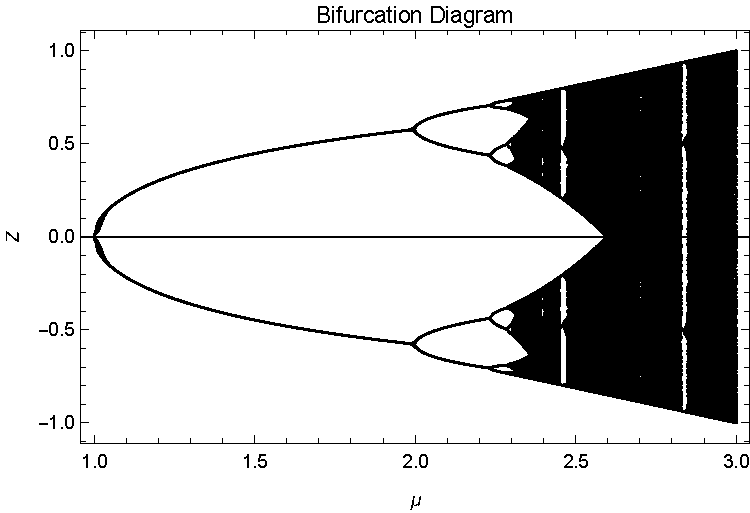
\includegraphics[height=0.4\textheight]{sam_hicks/bifurcation.eps}
    \caption{Bifurcation diagram of the multiplier-accelerator model varying $\mu$ between 0.9 and 3. The plot constructed using 0.1 as an initial point is displayed in black and the plot constructed using -0.1 as the initial point is displayed in blue. The last 50 points given a 10000 iteration timeseries are displayed.}
    \label{mult_bifurcation}
\end{figure}
Figure \ref{mult_bifurcation} displays the transitions this mapping makes between a stable fixed point, a 2-cycle, 4-cycle and so on until chaotic behavior arises. It is important to note though that even in the chaotic region, there exist windows of order. 
\begin{figure}
    \centering
    \includegraphics[height=0.4\textheight]{sam_hicks/unbound_cyclic.eps}
    \caption{Cobweb plot of the multiplier-accelerator model displaying a cycle featuring growth and decay. $\mu=2.7$ and $\dot Y_0=0.1$}
    \label{mult_unbound-cycle}
\end{figure}
Figure \ref{mult_unbound-cycle} displays a stable cycle that arises in one such window of order. This cycle is not bounded within its quadrant, it can thus feature endogenous growth and decay in the same cyclic trajectory, which is a significant distinction from all other cycles displayed thus far. 

Although the Feigenbaum point provides sufficient proof of the presence of chaos, it is still useful to plot the Lyapunov exponent in order to determine the exact regions of chaotic behavior.
\begin{figure}
    \centering
    \includegraphics[height=0.4\textheight]{sam_hicks/Lyapunov.eps}
    \caption{Plot of Lyapunov exponent varying $\mu$ using 0.1 as the initial point. $100,000^{th}$ iteration of the mapping is used to computationally solve for the Lyapunov exponent. }
    \label{mult_Lyapunov}
\end{figure}
Figure \ref{mult_Lyapunov} allows us to explicitly identify the parameter ranges of windows of order in the region of chaos. 